\documentclass[../MasterThesis.tex]{subfiles}
\graphicspath{ {./assets/images/} }
\captionsetup[figure]{list=no}




%----------------------------------------------------------------------------
%----------------------------------------------------------------------------

\begin{document}
	
	
\newpage

\section{README} \label{appendix:readme}


\subsection{Accurate-Player-3} \label{appendix:readmeaccurateplayer}

The README-file of the Accurate-Player-3 code was referenced as~\cite{RM_Frontend} and is included for transparency in the following.

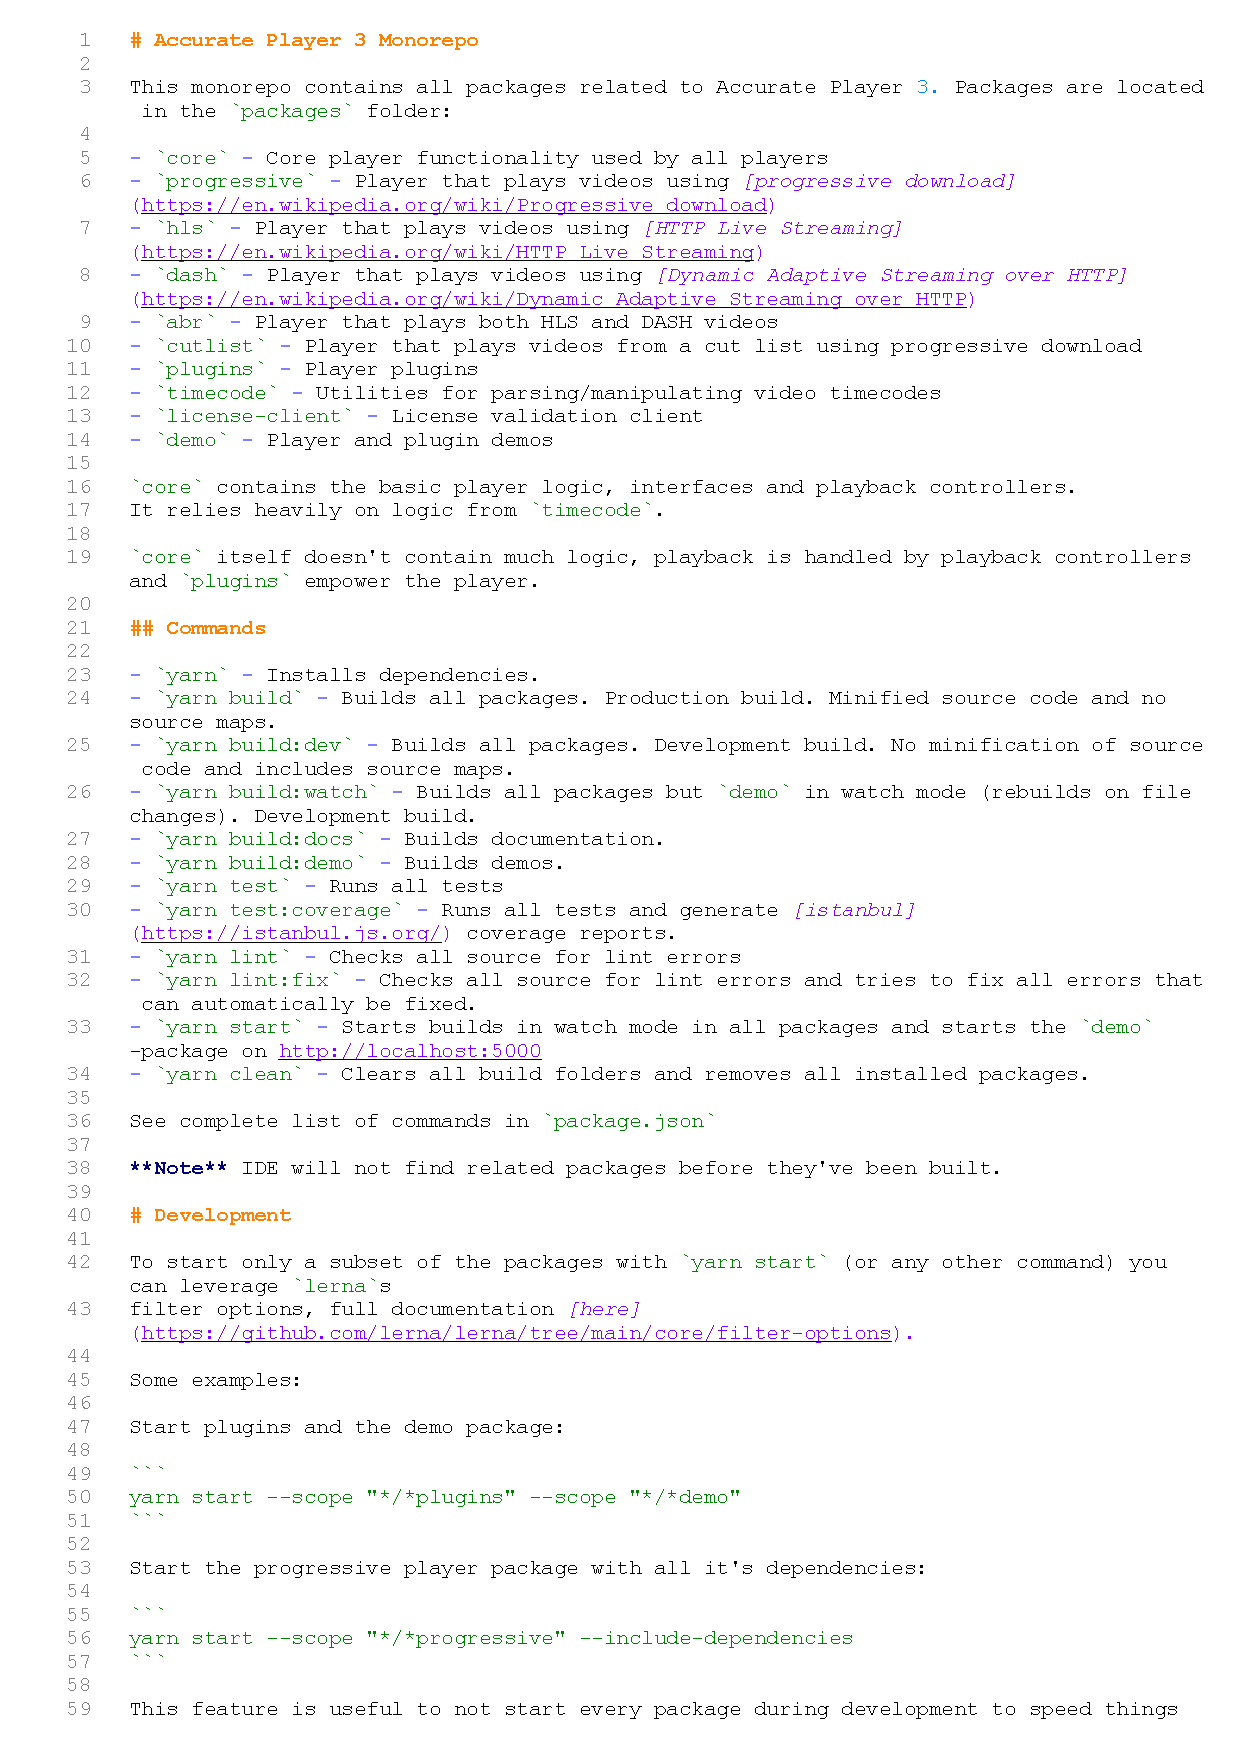
\includegraphics[page=1, width=0.9\textwidth]{FE.pdf}

\includegraphics[page=2, width=0.9\textwidth]{FE.pdf}



\newpage
\subsection{JIT-WebRTC} \label{appendix:readmejitwebrtc}

The README-file of the JIT-WebRTC code was referenced as~\cite{RM_Backend} and is included for transparency in the following.

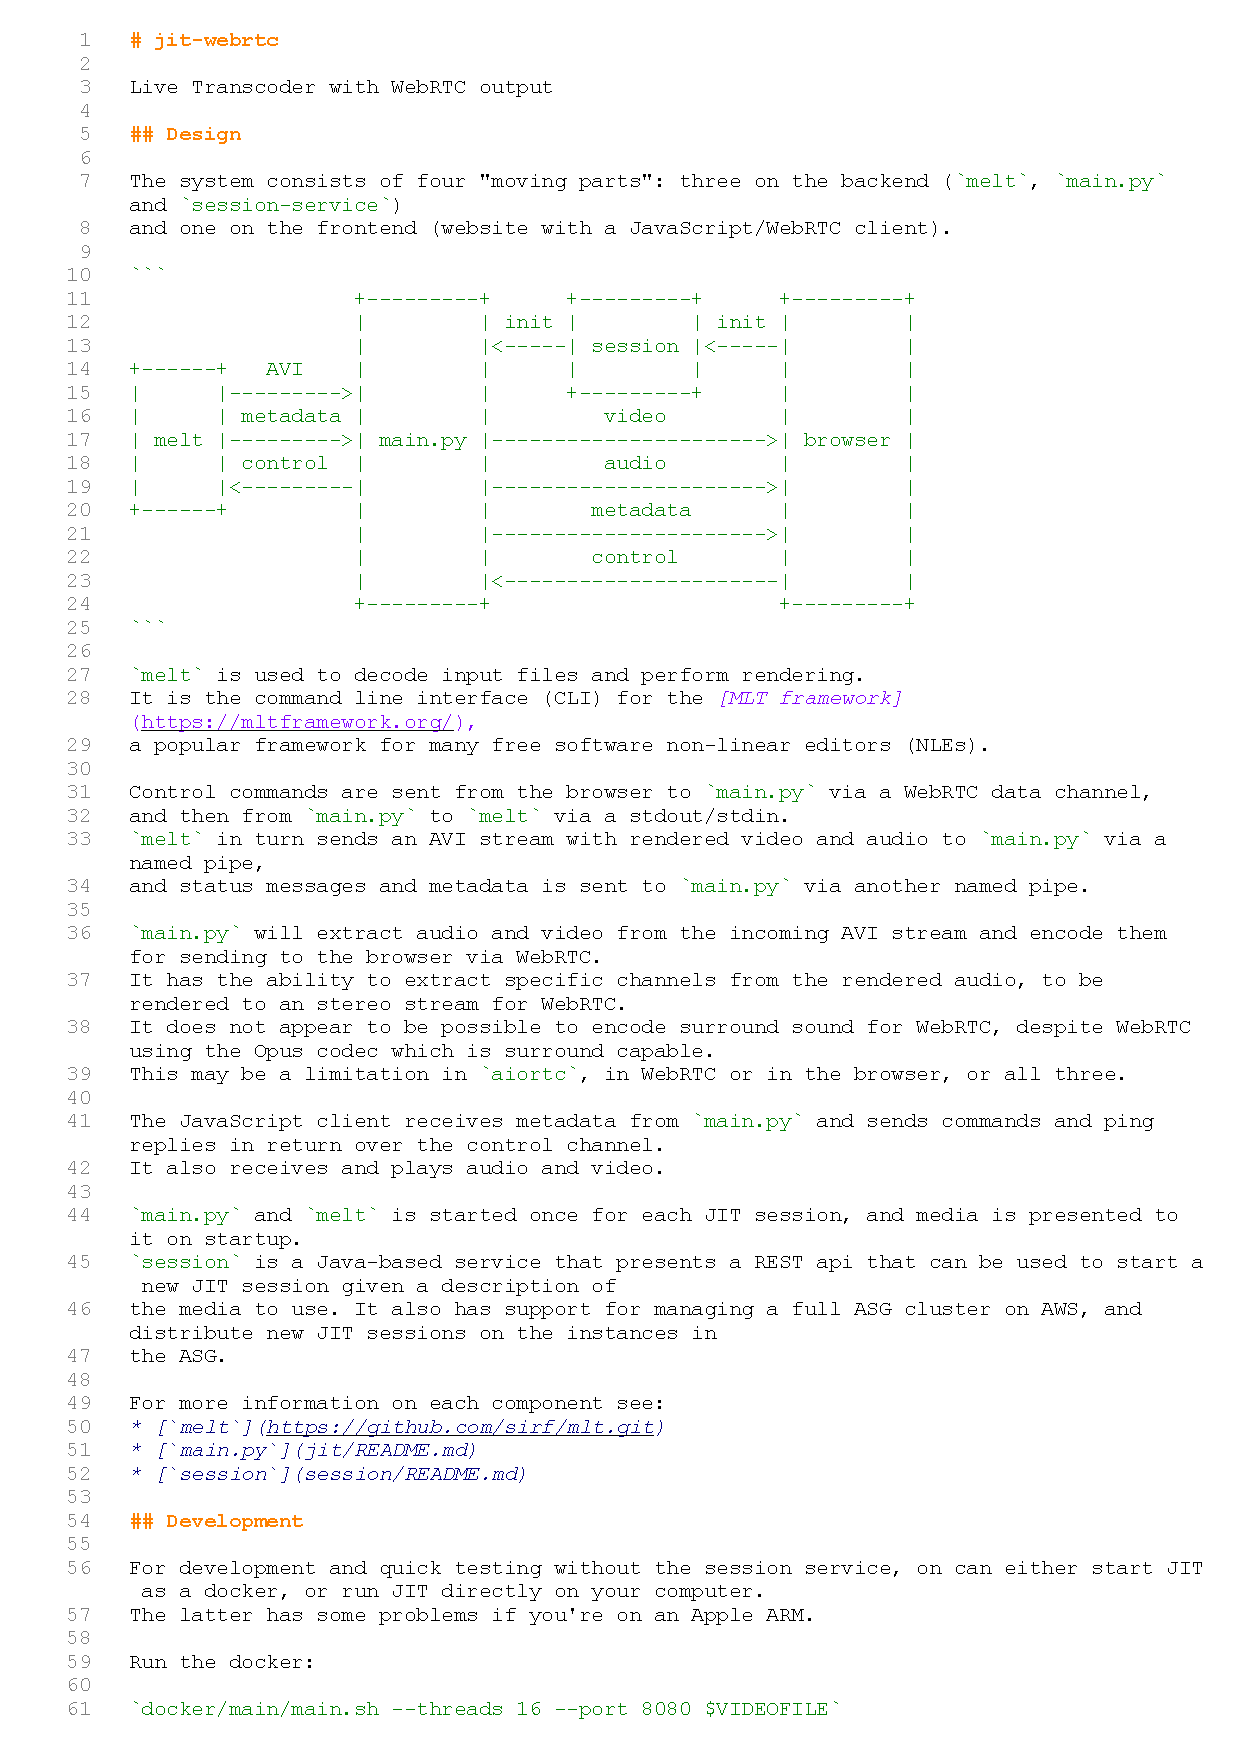
\includegraphics[page=1, width=0.9\textwidth]{BE.pdf}

\includegraphics[page=2, width=0.9\textwidth]{BE.pdf}












%----------------------------------------------------------------------------
%----------------------------------------------------------------------------

\newpage
\section{Comparison on all Colour Channels} \label{appendix:comparisonRGB}

%\captionsetup{font=small}

%\renewcommand{\captionfont}{\small} % Set caption font size to small
%\renewcommand{\captionlabelfont}{\bfseries} % Set caption label font to bold
\setlength{\abovecaptionskip}{2pt} % Adjust the space between caption and figure/table
\setlength{\belowcaptionskip}{4pt} % Adjust the space below caption
%\setlength{\baselineskip}{0.6\baselineskip} % Adjust the spacing between lines of captions

\vspace*{-0.4em}

\subsection*{Comparison with Melt}

\label{appendix:comparisonMelt}

\vspace*{-0.4em}

% RED

\textbf{Red}

\vspace*{-1.4em}

\begin{minipage}{0.48\textwidth}
	
	\begin{figure}[H]
		\begin{center}
			\cutpic{0.3cm}{0.99\textwidth}{red_Melt.jpg}
			\caption[]{\small Frame 343 after the application of the maximum value for red in Melt.}
			%\label{figure:redMelt}
		\end{center}
	\end{figure}
\end{minipage}\begin{minipage}{0.04\textwidth}
	\ 
\end{minipage}\begin{minipage}{0.48\textwidth}
	
	\begin{figure}[H]
		\begin{center}
			\cutpic{0.3cm}{0.99\textwidth}{red_AP.jpg}
			\caption[]{\small Frame 343 after the application of the maximum value for red in the Accurate Player.}
			%\label{figure:redAP}
		\end{center}
	\end{figure}
\end{minipage}

\vspace*{-1em}

\begin{figure}[H]
	\begin{center}
		\cutpic{0.3cm}{0.4752\textwidth}{filterVSfilter.jpg}
		\caption[]{\small Subtraction of the same frame with filter application: Melt frame is subtracted from the frame of the Accurate Player.}
		% JIT - Melt
		% \label{figure:filterVSfilter}
	\end{center}
\end{figure}



\vspace*{-1em}


% GREEN

\textbf{Green}

\vspace*{-1em}

\begin{minipage}{0.48\textwidth}
	
	\begin{figure}[H]
		\begin{center}
			\cutpic{0.3cm}{0.99\textwidth}{green_Melt.png}
			\caption[]{\small Frame 343 after the application of the maximum value for green in Melt.}
			%\label{figure:redMelt}
		\end{center}
	\end{figure}
\end{minipage}\begin{minipage}{0.04\textwidth}
	\ 
\end{minipage}\begin{minipage}{0.48\textwidth}
	
	\begin{figure}[H]
		\begin{center}
			\cutpic{0.3cm}{0.99\textwidth}{green_AP.png}
			\caption[]{\small Frame 343 after the application of the maximum value for green in the Accurate Player.}
			%\label{figure:redAP}
		\end{center}
	\end{figure}
\end{minipage}

\vspace*{-1em}

\begin{figure}[H]
	\begin{center}
		\cutpic{0.3cm}{0.4752\textwidth}{filterVSfilterG.png}
		\caption[]{\small Subtraction of the same frame with filter application: Melt frame is subtracted from the frame of the Accurate Player.}
		% JIT - Melt
		% \label{figure:filterVSfilter}
	\end{center}
\end{figure}








% BLUE

\textbf{Blue}

\vspace*{-1em}

\begin{minipage}{0.48\textwidth}
	
	\begin{figure}[H]
		\begin{center}
			\cutpic{0.3cm}{0.99\textwidth}{blue_Melt.png}
			\caption[]{\small Frame 343 after the application of the maximum value for blue in Melt.}
			%\label{figure:redMelt}
		\end{center}
	\end{figure}
\end{minipage}\begin{minipage}{0.04\textwidth}
	\ 
\end{minipage}\begin{minipage}{0.48\textwidth}
	
	\begin{figure}[H]
		\begin{center}
			\cutpic{0.3cm}{0.99\textwidth}{blue_AP.png}
			\caption[]{\small Frame 343 after the application of the maximum value for blue in the Accurate Player.}
			%\label{figure:redAP}
		\end{center}
	\end{figure}
\end{minipage}

\vspace*{-1em}

\begin{figure}[H]
	\begin{center}
		\cutpic{0.3cm}{0.4752\textwidth}{filterVSfilterB.png}
		\caption[]{\small Subtraction of the same frame with filter application: Melt frame is subtracted from the frame of the Accurate Player.}
		% JIT - Melt
		% \label{figure:filterVSfilter}
	\end{center}
\end{figure}














% \newpage

\subsection*{Comparison with KDEN Live}

\label{appendix:comparisonKDENLive}

\vspace*{-0.4em}

\subsubsection*{Change gamma}

\vspace*{-0.4em}

% RED

\textbf{Red}

\vspace*{-1em}

\begin{minipage}{0.48\textwidth}
	\begin{figure}[H]
		\begin{center}
			\cutpic{0.3cm}{0.99\textwidth}{red_AP.jpg}
			\caption[]{\small Frame 343 after the application of the maximum value for red in the Accurate Player.}
			%\label{figure:APframe1}
		\end{center}
	\end{figure}
\end{minipage}\begin{minipage}{0.04\textwidth}
	\ 
\end{minipage}\begin{minipage}{0.48\textwidth}
	\begin{figure}[H]
		\begin{center}
			\cutpic{0.3cm}{0.99\textwidth}{gamma.png}
			\caption[]{\small Frame 343 from KDEN Live with the action \textit{change gamma} in the red filter application.}
			%\label{figure:gamma}
		\end{center}
	\end{figure}
\end{minipage}

\vspace*{-1em}

\begin{figure}[H]
	\begin{center}
		\cutpic{0.3cm}{0.4752\textwidth}{gamma_gimp.png}
		\caption[]{\small Subtraction of the two frames: Accurate Player frame is subtracted from the KDEN Live frame (with the action \textit{change gamma}).}
		% KDENLive - JIT
		%\label{figure:gammagimp}
	\end{center}
\end{figure}






% GREEN
\vspace*{-1em}

\textbf{Green}

\vspace*{-1em}

\begin{minipage}{0.48\textwidth}
	\begin{figure}[H]
		\begin{center}
			\cutpic{0.3cm}{0.99\textwidth}{green_AP.png}
			\caption[]{\small Frame 343 after the application of the maximum value for green in the Accurate Player.}
			%\label{figure:APframe1}
		\end{center}
	\end{figure}
\end{minipage}\begin{minipage}{0.04\textwidth}
	\ 
\end{minipage}\begin{minipage}{0.48\textwidth}
	\begin{figure}[H]
		\begin{center}
			\cutpic{0.3cm}{0.99\textwidth}{g_gamma.png}
			\caption[]{\small Frame 343 from KDEN Live with the action \textit{change gamma} in the green filter application.}
			%\label{figure:gamma}
		\end{center}
	\end{figure}
\end{minipage}

\vspace*{-1em}

\begin{figure}[H]
	\begin{center}
		\cutpic{0.3cm}{0.4752\textwidth}{gamma_gimp_g.png}
		\caption[]{\small Subtraction of the two frames: Accurate Player frame is subtracted from the KDEN Live frame (with the action \textit{change gamma}).}
		% KDENLive - JIT
		%\label{figure:gammagimp}
	\end{center}
\end{figure}







\vspace*{-1em}

% BLUE
\textbf{Blue}

\vspace*{-1em}


\begin{minipage}{0.48\textwidth}
	\begin{figure}[H]
		\begin{center}
			\cutpic{0.3cm}{0.99\textwidth}{blue_AP.png}
			\caption[]{\small Frame 343 after the application of the maximum value for blue in the Accurate Player.}
			%\label{figure:APframe1}
		\end{center}
	\end{figure}
\end{minipage}\begin{minipage}{0.04\textwidth}
	\ 
\end{minipage}\begin{minipage}{0.48\textwidth}
	\begin{figure}[H]
		\begin{center}
			\cutpic{0.3cm}{0.99\textwidth}{b_gamma.png}
			\caption[]{\small Frame 343 from KDEN Live with the action \textit{change gamma} in the blue filter application.}
			%\label{figure:gamma}
		\end{center}
	\end{figure}
\end{minipage}

\vspace*{-1em}

\begin{figure}[H]
	\begin{center}
		\cutpic{0.3cm}{0.4752\textwidth}{gamma_gimp_b.png}
		\caption[]{\small Subtraction of the two frames: Accurate Player frame is subtracted from the KDEN Live frame (with the action \textit{change gamma}).}
		% KDENLive - JIT
		%\label{figure:gammagimp}
	\end{center}
\end{figure}















\subsubsection*{Add constant}




% RED
\textbf{Red}

\vspace*{-1em}

\begin{minipage}{0.48\textwidth}
	\begin{figure}[H]
		\begin{center}
			\cutpic{0.3cm}{0.99\textwidth}{red_AP.jpg}
			\caption[]{\small Frame 343 after the application of the maximum value for red in the Accurate Player.}
			% \label{figure:APframe2}
		\end{center}
	\end{figure}
\end{minipage}\begin{minipage}{0.04\textwidth}
	\ 
\end{minipage}\begin{minipage}{0.48\textwidth}
	\begin{figure}[H]
		\begin{center}
			\cutpic{0.3cm}{0.99\textwidth}{addconstant.png}
			\caption[]{\small Frame 343 from KDEN Live with the action \textit{add constant} in the red filter application.}
			% \label{figure:addconstant}
		\end{center}
	\end{figure}
\end{minipage}

\vspace*{-1em}

\begin{figure}[H]
	\begin{center}
		\cutpic{0.3cm}{0.4752\textwidth}{addconstant_gimp.png}
		\caption[]{\small Subtraction of the two frames: Accurate Player frame is subtracted from the KDEN Live frame extraction (with the action \textit{add constant}).}
		% KDENLive - JIT
		% \label{figure:addconstantgimp}
	\end{center}
\end{figure}





\vspace*{-1em}
% GREEN 
\textbf{Green}

\vspace*{-1em}


\begin{minipage}{0.48\textwidth}
	\begin{figure}[H]
		\begin{center}
			\cutpic{0.3cm}{0.99\textwidth}{green_AP.png}
			\caption[]{\small Frame 343 after the application of the maximum value for green in the Accurate Player.}
			% \label{figure:APframe2}
		\end{center}
	\end{figure}
\end{minipage}\begin{minipage}{0.04\textwidth}
	\ 
\end{minipage}\begin{minipage}{0.48\textwidth}
	\begin{figure}[H]
		\begin{center}
			\cutpic{0.3cm}{0.99\textwidth}{g_addconstant.png}
			\caption[]{\small Frame 343 from KDEN Live with the action \textit{add constant} in the green filter application.}
			% \label{figure:addconstant}
		\end{center}
	\end{figure}
\end{minipage}

\vspace*{-1em}

\begin{figure}[H]
	\begin{center}
		\cutpic{0.3cm}{0.4752\textwidth}{addconstant_gimp_g.png}
		\caption[]{\small Subtraction of the two frames: Accurate Player frame is subtracted from the KDEN Live frame extraction (with the action \textit{add constant}).}
		% KDENLive - JIT
		% \label{figure:addconstantgimp}
	\end{center}
\end{figure}



\vspace*{-1em}


% BLUE
\textbf{Blue}

\vspace*{-1em}


\begin{minipage}{0.48\textwidth}
	\begin{figure}[H]
		\begin{center}
			\cutpic{0.3cm}{0.99\textwidth}{blue_AP.png}
			\caption[]{\small Frame 343 after the application of the maximum value for blue in the Accurate Player.}
			% \label{figure:APframe2}
		\end{center}
	\end{figure}
\end{minipage}\begin{minipage}{0.04\textwidth}
	\ 
\end{minipage}\begin{minipage}{0.48\textwidth}
	\begin{figure}[H]
		\begin{center}
			\cutpic{0.3cm}{0.99\textwidth}{b_addconstant.png}
			\caption[]{\small Frame 343 from KDEN Live with the action \textit{add constant} in the green filter application.}
			% \label{figure:addconstant}
		\end{center}
	\end{figure}
\end{minipage}

\vspace*{-1em}



\begin{figure}[H]
	\begin{center}
		\cutpic{0.3cm}{0.4752\textwidth}{addconstant_gimp_b.png}
		\caption[]{\small Subtraction of the two frames: Accurate Player frame is subtracted from the KDEN Live frame extraction (with the action \textit{add constant}).}
		% KDENLive - JIT
		% \label{figure:addconstantgimp}
	\end{center}
\end{figure}

















\subsubsection*{Multiply}


% RED
\textbf{Red}

\vspace*{-1em}


\begin{minipage}{0.48\textwidth}
	\begin{figure}[H]
		\begin{center}
			\cutpic{0.3cm}{0.99\textwidth}{red_AP.jpg}
			\caption[]{\small Frame 343 after the application of the maximum value for red in the Accurate Player.}
			% \label{figure:APframe3}
		\end{center}
	\end{figure}
\end{minipage}\begin{minipage}{0.04\textwidth}
	\ 
\end{minipage}\begin{minipage}{0.48\textwidth}
	\begin{figure}[H]
		\begin{center}
			\cutpic{0.3cm}{0.99\textwidth}{multiply.png}
			\caption[]{\small Frame 343 from KDEN Live with the action \textit{Multiply} in the red filter application.}
			% \label{figure:multiply}
		\end{center}
	\end{figure}
\end{minipage}

\vspace*{-1em}

\begin{figure}[H]
	\begin{center}
		\cutpic{0.3cm}{0.4752\textwidth}{multiply_gimp.png}
		\caption[]{\small Subtraction of the two frames: Accurate Player frame is subtracted from the KDEN Live frame extraction (with the action \textit{Multiply}).}
		% KDEN Live - JIT
		%\label{figure:multiplygimp}
	\end{center}
\end{figure}




\vspace*{-1em}
% GREEN
\textbf{Green}

\vspace*{-1em}


\begin{minipage}{0.48\textwidth}
	\begin{figure}[H]
		\begin{center}
			\cutpic{0.3cm}{0.99\textwidth}{green_AP.png}
			\caption[]{\small Frame 343 after the application of the maximum value for green in the Accurate Player.}
			% \label{figure:APframe3}
		\end{center}
	\end{figure}
\end{minipage}\begin{minipage}{0.04\textwidth}
	\ 
\end{minipage}\begin{minipage}{0.48\textwidth}
	\begin{figure}[H]
		\begin{center}
			\cutpic{0.3cm}{0.99\textwidth}{g_multiply.png}
			\caption[]{\small Frame 343 from KDEN Live with the action \textit{Multiply} in the green filter application.}
			% \label{figure:multiply}
		\end{center}
	\end{figure}
\end{minipage}

\vspace*{-1em}

\begin{figure}[H]
	\begin{center}
		\cutpic{0.3cm}{0.4752\textwidth}{multiply_gimp_g.png}
		\caption[]{\small Subtraction of the two frames: Accurate Player frame is subtracted from the KDEN Live frame extraction (with the action \textit{Multiply}).}
		% KDEN Live - JIT
		%\label{figure:multiplygimp}
	\end{center}
\end{figure}


\vspace*{-1em}

% BLUE
\textbf{Blue}

\vspace*{-1em}


\begin{minipage}{0.48\textwidth}
	\begin{figure}[H]
		\begin{center}
			\cutpic{0.3cm}{0.99\textwidth}{blue_AP.png}
			\caption[]{\small Frame 343 after the application of the maximum value for blue in the Accurate Player.}
			% \label{figure:APframe3}
		\end{center}
	\end{figure}
\end{minipage}\begin{minipage}{0.04\textwidth}
	\ 
\end{minipage}\begin{minipage}{0.48\textwidth}
	\begin{figure}[H]
		\begin{center}
			\cutpic{0.3cm}{0.99\textwidth}{b_multiply.png}
			\caption[]{\small Frame 343 from KDEN Live with the action \textit{Multiply} in the blue filter application.}
			% \label{figure:multiply}
		\end{center}
	\end{figure}
\end{minipage}

\vspace*{-1em}

\begin{figure}[H]
	\begin{center}
		\cutpic{0.3cm}{0.4752\textwidth}{multiply_gimp_b.png}
		\caption[]{\small Subtraction of the two frames: Accurate Player frame is subtracted from the KDEN Live frame extraction (with the action \textit{Multiply}).}
		% KDEN Live - JIT
		%\label{figure:multiplygimp}
	\end{center}
\end{figure}








%----------------------------------------------------------------------------
%----------------------------------------------------------------------------

\newpage
\section{Different MLT Filters} \label{appendix:differentMeltFilter}

In the following, different MLT filters that influence the visual appearance of a video are listed. This list does not contain every filter and the applied parameters for the different filter results vary. This is not a complete listing or analysis of the MLT filters but an overview over many of the filters and the options that arise from combining them or adapting the parameters. The complete list of filters without visual examples can be found on the MLT web site~\cite{melt_filters}.
%
\begin{figure}[H]
	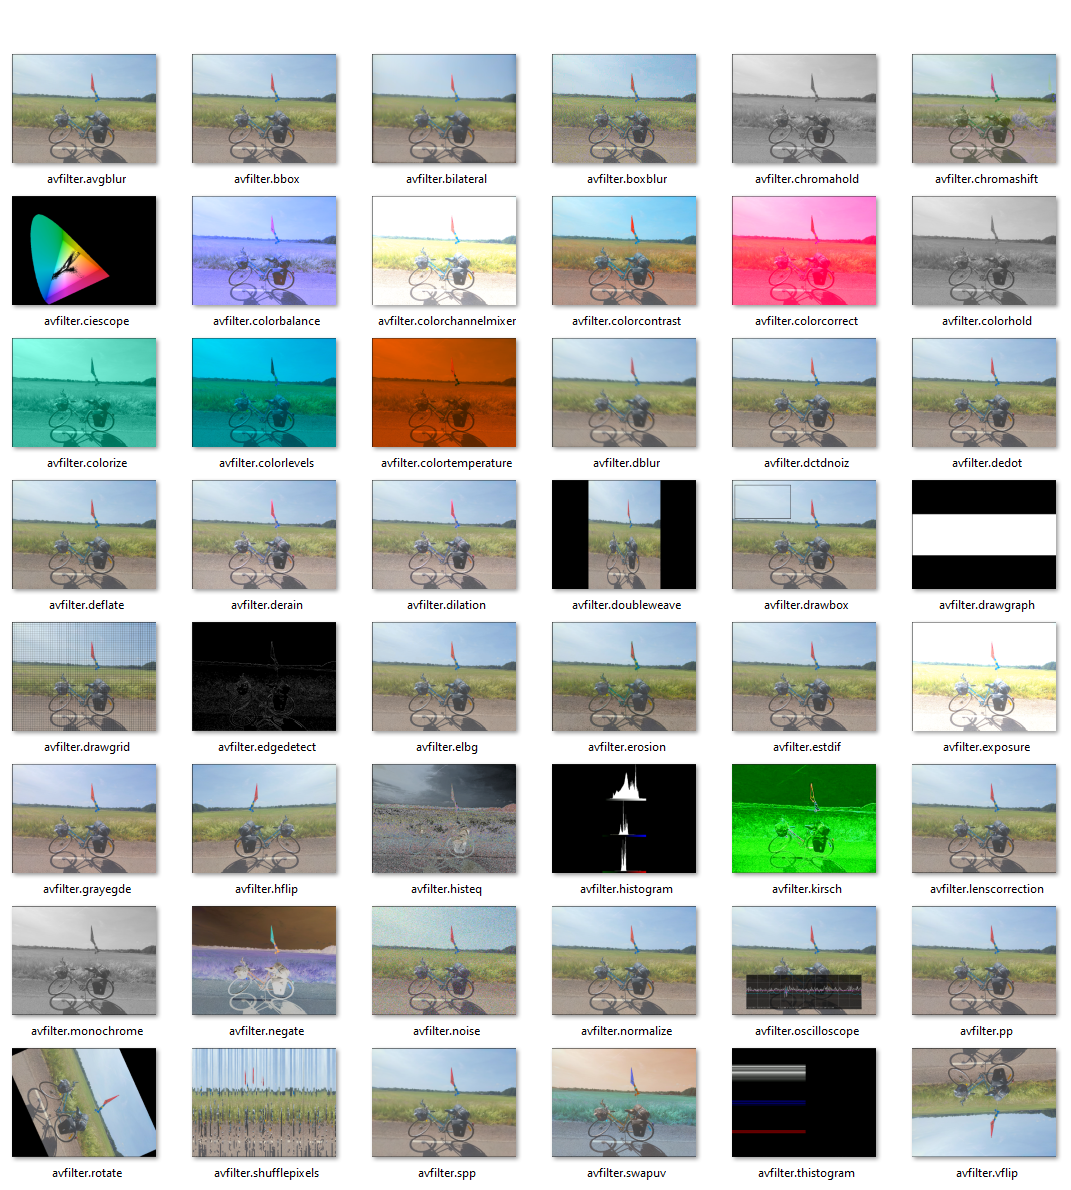
\includegraphics[width=1\textwidth]{Seite1.png}
\end{figure}

\begin{figure}[H]
	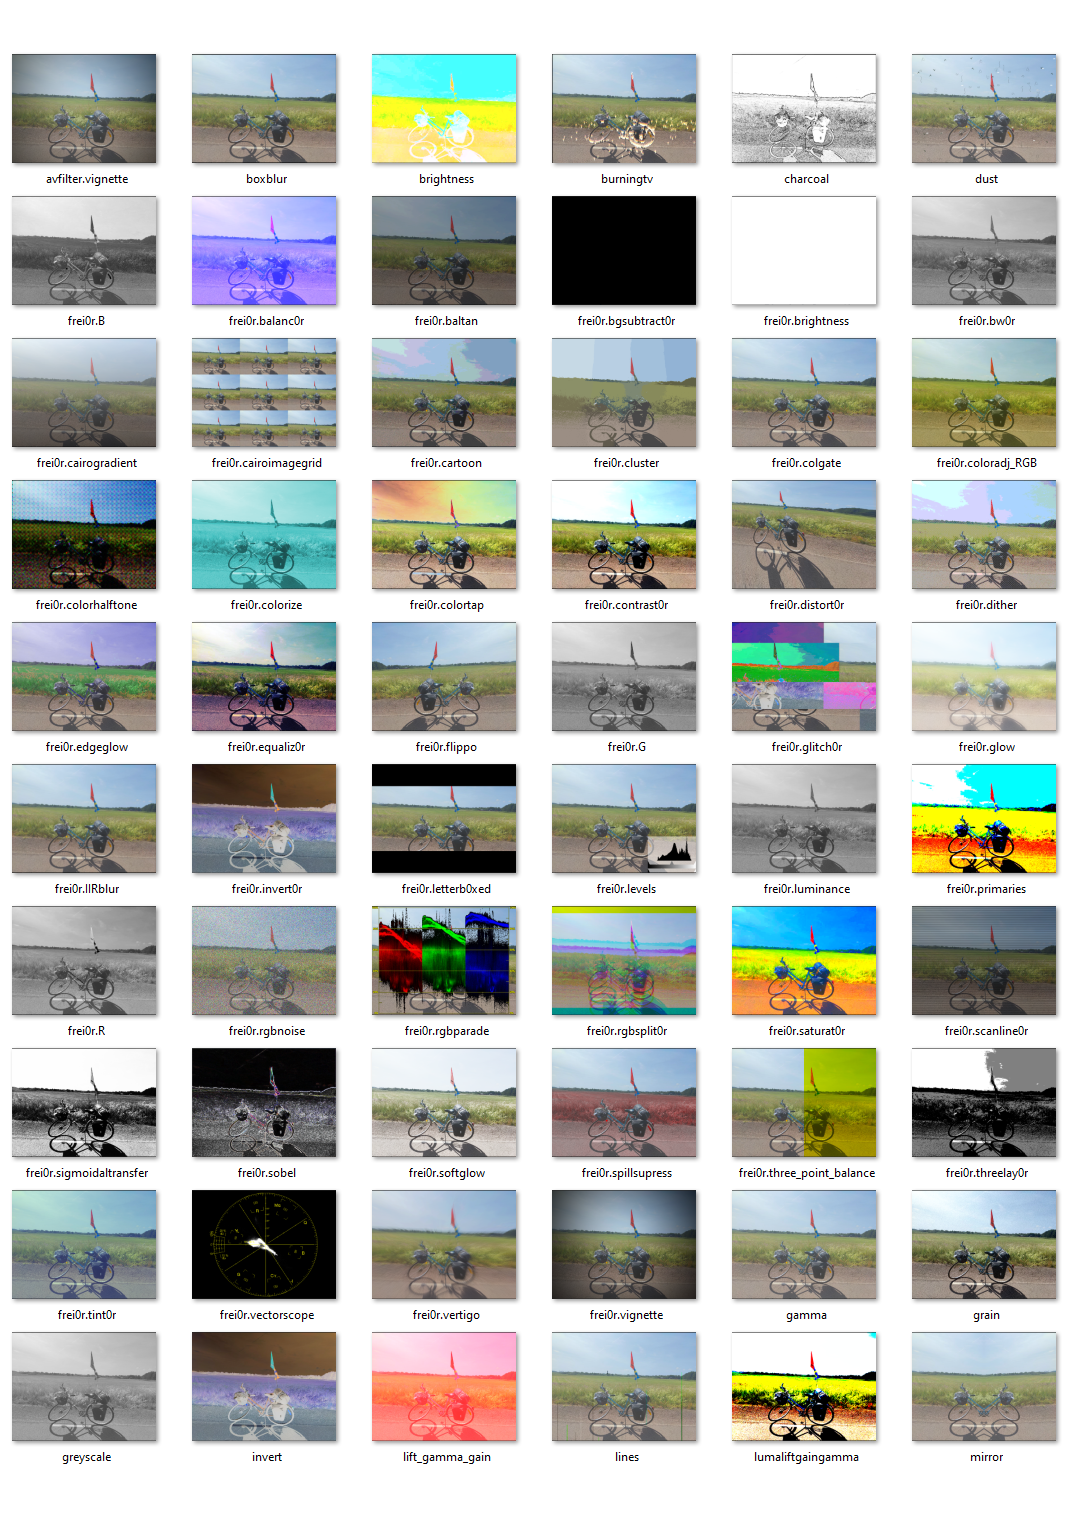
\includegraphics[width=1\textwidth]{Seite2.png}
\end{figure}

\begin{figure}[H]
	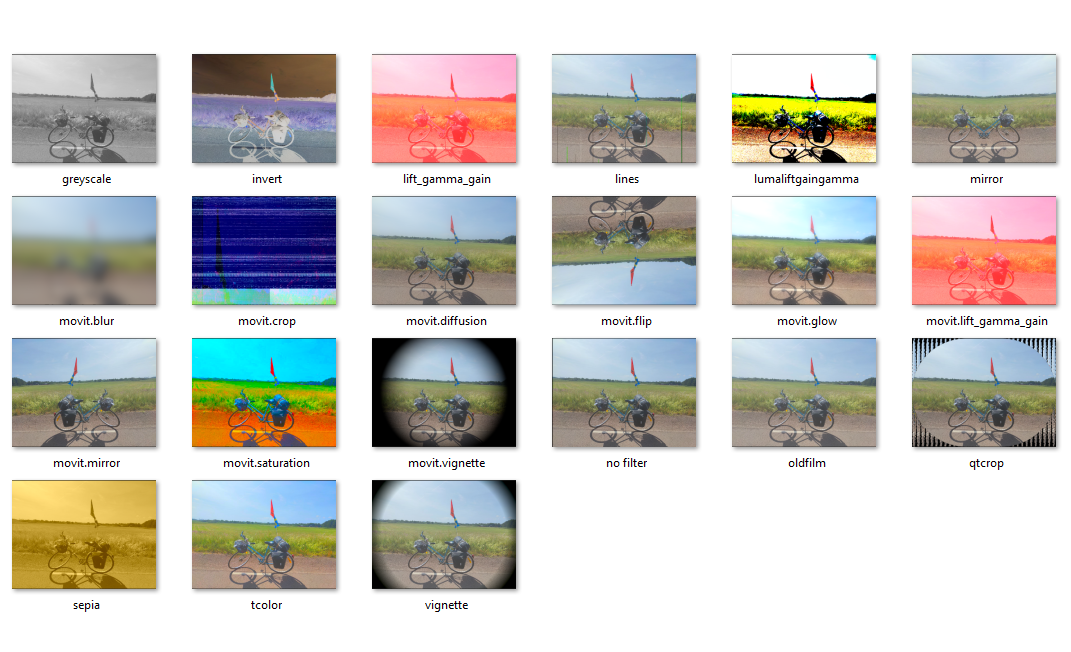
\includegraphics[width=1\textwidth]{Seite3.png}
\end{figure}







	
	
\end{document}